\textbf{1-1} 半圆柱形玻璃的折射率 $n = \sqrt{2}$，放置在空气中。在垂直于半圆柱体轴的平面内，光线以 $45^{\circ}$ 角入射在半圆柱体的平表面上。试问光线从半圆柱体的什么范围内透出（以角度表示）。
\vfill

\textbf{1-2} 如光图1-2-1所示，在内半径为 $r$，外半径为 $R$，折射率为 $n_1$ 的玻璃管内充满了折射率为 $n_2$ 的发光液体。试问，从远处看，当管的厚度消失时，$r$ 和 $R$ 应满足什么条件。

\begin{center}
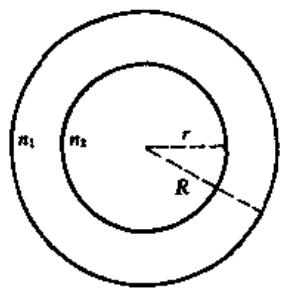
\includegraphics[width=0.3\textwidth]{figures/光图1-2-1.jpg}
\end{center}
\vfill

\newpage
\textbf{1-3} 如光图1-3-1所示，一条光线射入空气中的球状水滴，在水滴内表面反射后又穿出水滴。入射光线与出射光线之间的夹角 $\delta$ 称为偏向角。已知水滴的折射率为 $n$。试问：

1. 光线在水滴内表面反射时是全反射还是部分反射；

2. 当偏向角为最小偏向角时，入射光线的入射角 $\theta$ 应满足什么条件。
\begin{center}
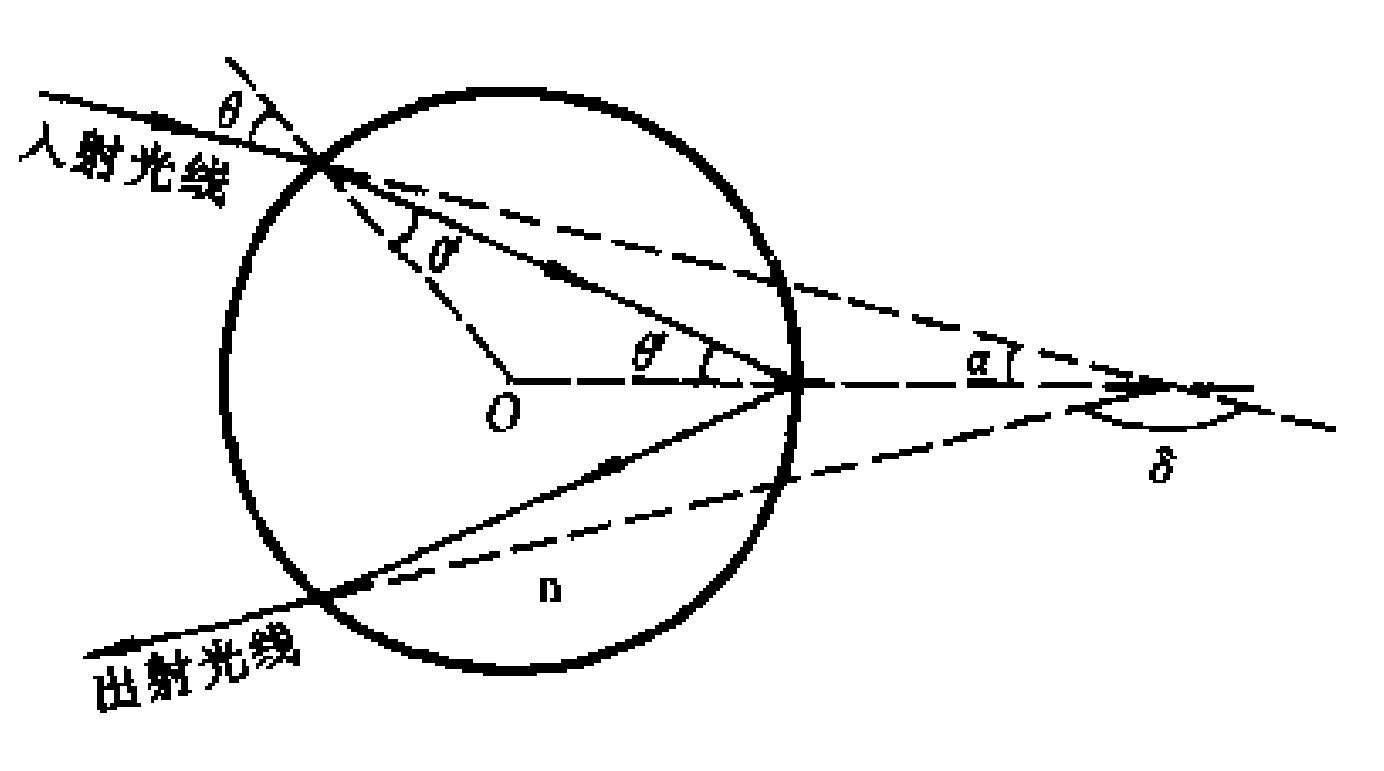
\includegraphics[width=0.3\textwidth]{figures/光图1-3-1.jpg}
\end{center}
\vfill

\textbf{1-4} 1. 设温度计由圆柱形玻璃管做成，内、外直径分别为 $2r = 1\,\mathrm{mm}$ 和 $2R = 3\,\mathrm{mm}$，玻璃折射率 $n_1 = 1.5$，空气折射率 $n_2 = 1$。试问当从侧面远处观察时，内直径的表观尺寸是多少？

2. 某温度计的外直径和玻璃的折射率都与上述温度计相同，但内直径 $2r = 0.1\,\mathrm{mm}$。将此温度计垂直悬挂于盛水玻璃烧杯的中心位置，水的折射率为 $n_1' = \frac{4}{3}$。试问当从烧杯外远处观察时，温度计内、外直径的表观尺寸是多少？
\vfill

\newpage
\textbf{1-5} 如光图1-5-1所示，两平面反射镜A和B斜交，交棱为O，两镜夹角为 $\theta$，两反射镜的反射面相对。在两反射镜之间有一物点 $P$，从 $P$ 点向交棱作垂线OP，OP与两镜的夹角分别为 $\alpha$ 和 $\beta$，观察者位于A和B两镜之间。

试求观察者能看到物点 $P$ 的像的个数及各像的位置。

\begin{center}
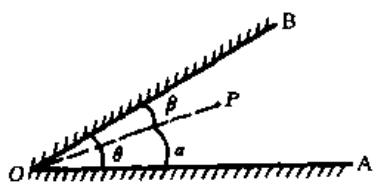
\includegraphics[width=0.3\textwidth]{figures/光图1-5-1.jpg}
\end{center}
\vfill

\textbf{1-6} 如光图1-6-1所示，等腰玻璃三棱镜的折射率 $n = 1.50$，顶部截去，底部浸在水中，水的折射率 $n_{\text{水}} = 1.33$，入射的平行光与底面平行。

试求出射光线的偏向角。

\begin{center}
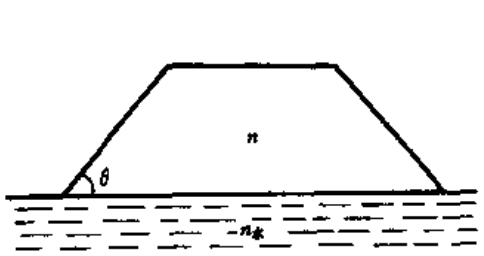
\includegraphics[width=0.3\textwidth]{figures/光图1-6-1.jpg}
\end{center}
\vfill

\newpage
\textbf{1-7} 已知飞机场跑道上空空气的折射率随高度 $y$ 变化的规律为
$$
n = n_0(1 + \alpha y)
$$
式中 $n_0$ 为地表空气折射率，$\alpha$ 为正常数。一飞机在跑道上空沿平行于地面的方向以速度 $v$ 飞行，试求从飞机上发出的无线电信号传到地面所需的时间。
\vfill

\textbf{1-8} 如光图1-8-1所示，平板玻璃的折射率 $n$ 随 $x$ 变化的规律为
$$
n^2 = n_0^2(1 - \alpha^2 x^2)
$$
式中 $n_0$ 和 $\alpha$ 均为常量，$\alpha x \ll 1$。一束光线从玻璃板的左端面沿 $x$ 方向入射，入射处折射率为 $n_0$。试求光线在玻璃板中的传播轨迹。

\begin{center}
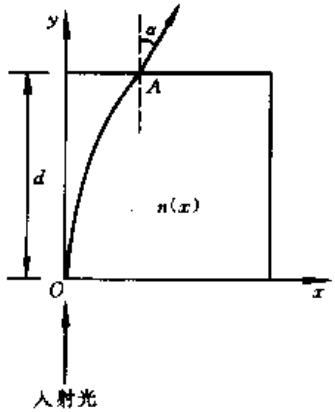
\includegraphics[width=0.25\textwidth]{figures/光图1-8-1.jpg}
\end{center}
\vfill

\newpage
\textbf{1-9} 白天沙漠上空的气温随高度 $y$ 增加而递减，下层空气温度较高，密度和折射率较小，上层空气则相反。这种折射率的不均匀分布造成了所谓海市蜃楼的光学现象。比较符合实际的折射率随高度变化的规律为
$$
n^2 = n_0^2(1 - 2\alpha y)
$$
式中 $n_0$ 为地面处空气折射率，$\alpha$ 为常量。试求光线在空气中传播的轨迹。
\vfill

\textbf{1-10} 在湿冷的海水上空，空气折射率随高度增加而递减，由于光线向下弯曲，会出现上现蜃景。空气折射率包括一常数项和另一随高度 $y$ 变化的项，为
$$
n^2 = n_0^2 + 2\alpha y
$$
式中 $\alpha > 0$。设地面附近海面上有一静止物体，试讨论能否观察到上现蜃景。
\vfill

\newpage
\textbf{1-11} 已知光学纤维的折射率 $n$ 沿径向的分布为
$$
n^2 = n_0^2(1 - \alpha^2 r^2)
$$
式中 $n_0$ 为中心的折射率，$\alpha$ 为比1小得多的正数。试求光线在纤维中传播的轨迹。
\vfill

\textbf{1-12} 如光图1-12-1所示，在半径为 $r$ 的球面两侧，介质的折射率分别为 $n_1$ 和 $n_2(n_1 < n_2)$，在主光轴上有一点光源 $Q$，它与球面顶点 $O$ 相距为 $s$，另一任意点 $Q'$ 与 $O$ 点相距为 $s'$。试问：在傍轴条件下，从 $Q$ 点发出的光线中哪些光线能到达 $Q'$ 点，其光程是极大、极小还是稳定值？$s$ 和 $s'$ 应满足什么条件，$Q'$ 才是 $Q$ 的像点。
\begin{center}
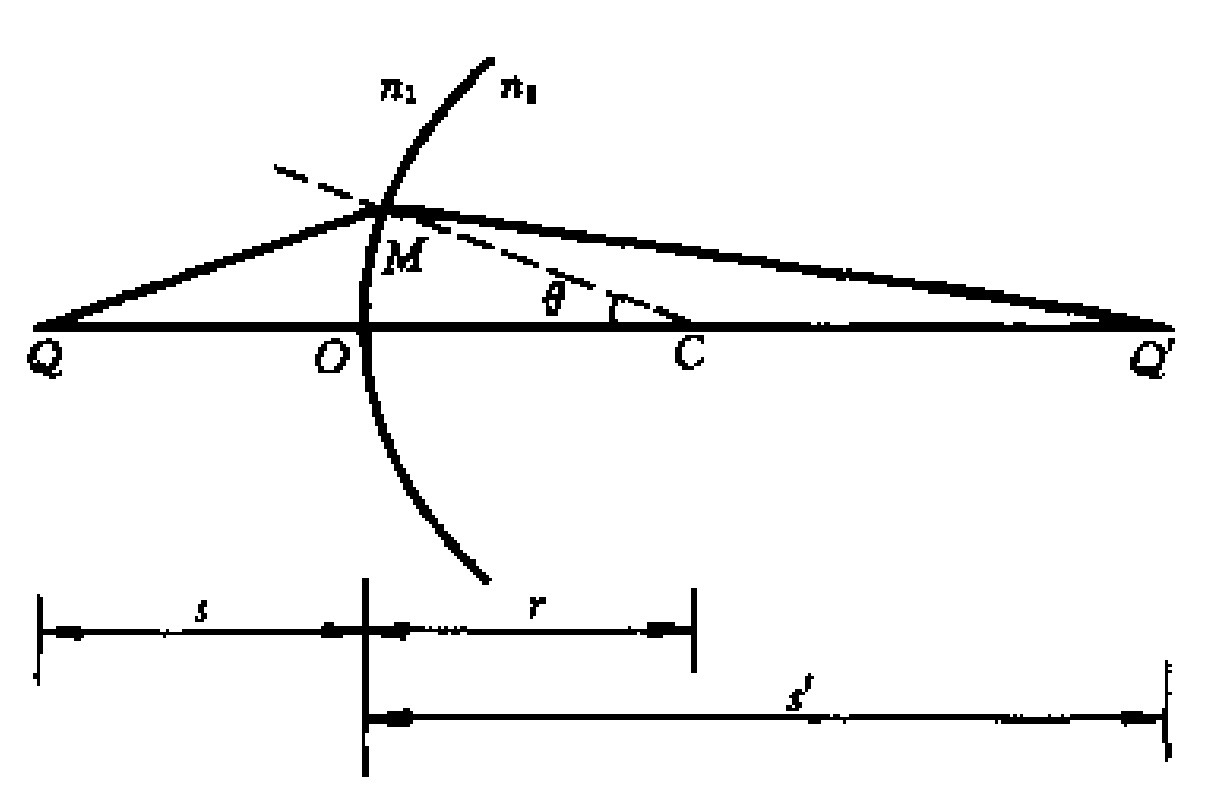
\includegraphics[width=0.3\textwidth]{figures/光图1-12-1.jpg}
\end{center}
\vfill

\newpage
\textbf{1-13} 如光图1-13-1所示，一平凸透镜的折射率为 $n$，放置在空气中。透镜孔径的半径为 $R$，在透镜外主光轴上取一点 $F$，$\overline{OF} = f$。当平行光沿主光轴入射时，为使所有光线都会聚在 $F$ 点，试问透镜凸面应取什么形状，透镜顶点 $A$ 点与 $O$ 点相距多少，对透镜的孔径 $R$ 有何限制。

\begin{center}
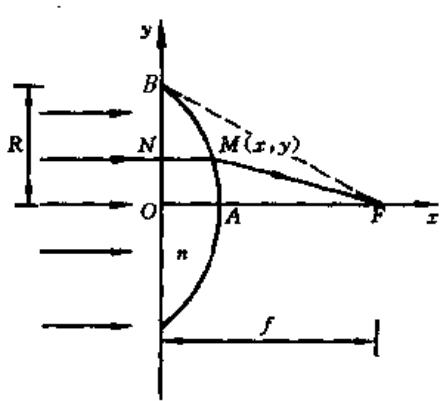
\includegraphics[width=0.3\textwidth]{figures/光图1-13-1.jpg}
\end{center}
\vfill

\textbf{1-14} 大气折射率 $n$ 与空气的密度有关，假设 $(n-1)$ 与密度 $\rho$ 成正比。由于大气密度遵从玻尔兹曼分布律，大气折射率将随高度的增加而递减，使得光线在大气中弯曲传播。为使光线能沿着地球表面的圆弧线弯曲传播，试问地表的空气密度应是实际密度的多少倍？

设大气层是等温的，温度 $T=300\,\mathrm{K}$。地表空气的实测折射率为 $n_0 = 1.0003$，空气的平均分子量 $\mu = 29$，地球半径为 $r_0 = 6400 \times 10^{3} m$。

\vfill
\newpage

\textbf{1-15} 球面透镜一般只对傍轴光线才能近似地成像，对于如光图1-15-1所示的弯月形透镜，当物点位于主光轴上的特殊点时，即使是非傍轴光线，经透镜折射后的出射光线均能交于同一点，即能理想成像。       如光图1-15-1的弯月形透镜, 透镜折射率为 $n$ , 放置在空气中, 它的两个球面 $\Sigma_1$ 和 $\Sigma_2$ 的球心分别为 $C_1$ 和 $C_2$ , 球面 $\Sigma_2$ 的半径为 $R_2$ . 已知 $\overline{C_1C_2} = \frac{R_2}{n}$ , 物点 $Q$ 位于 $C_1$ 点. 试证明从 $Q$ 点发出的任何光线 (包括非傍轴光线) 经透镜折射后, 出射光线都能相交于同一像点 $Q'$ .

\begin{center}
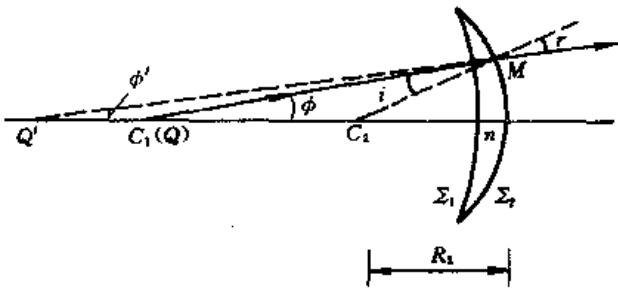
\includegraphics[width=0.3\textwidth]{figures/光图1-15-1.jpg}
\end{center}
\vfill


\textbf{1-16} 如光图1-16-1所示，薄壁球形玻璃鱼缸的半径为 $R$ ，所盛水的折射率 $n = \frac{4}{3}$ .鱼缸左侧与轴线垂直的平面反射镜离球心的距离为 $3R$ .一条位于左球面顶点处的小鱼沿缸壁以速  度 v 游动．从鱼缸右侧观察鱼的直接像与反射像（先经平面镜反射，再经鱼缸所成的像）．试求两像之间的相对速度．
\begin{center}
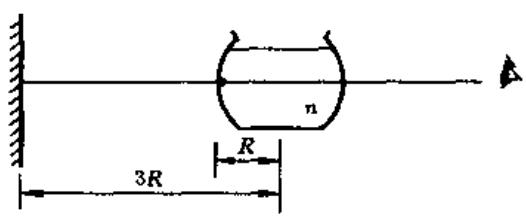
\includegraphics[width=0.3\textwidth]{figures/光图1-16-1.jpg}
\end{center}
\vfill
\newpage

\textbf{1-17} 如光图1-17-1所示，有一半径 $R = 0.128\mathrm{m}$ 的玻璃半球，在其主光轴上放一长 $l =$  0.020 m的条形物 $A_{1}A_{2}$ . 在 E 点附近可同时观察到 $A_{1}A_{2}$ 的两个像, 它们分别是经玻璃半球的平面和凹球面反射而得. 并且, 当条形物的 $A_{2}$ 端与半球平面相距 0.020 m 时, 两个像恰好连接在一起. 试求玻璃半球的折射率 n.

\begin{center}
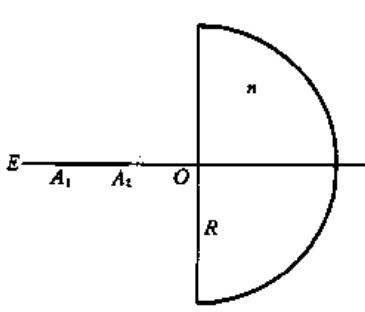
\includegraphics[width=0.3\textwidth]{figures/光图1-17-1.jpg}
\end{center}
\vfill


\textbf{1-18} 如光图1-18-1，已知杯高 $h_0 = 15\mathrm{cm}$ ，在杯底放一钱币，其直径 $D = 1.5\mathrm{cm}$ ，杯口放一薄凸透镜，它在空气中的焦距 $f = 10\mathrm{cm}$ ，杯中盛水，高度为 $h$ ，水的折射率 $n = \frac{4}{3}$ 。试求：在傍轴条件下，当 $h = 0.8h_0$ 时，钱币的像的位置和大小。

\begin{center}
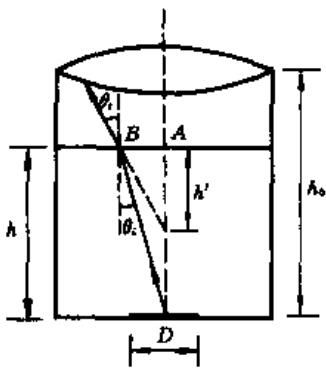
\includegraphics[width=0.3\textwidth]{figures/光图1-18-1.jpg}
\end{center}
\vfill
\newpage

\textbf{1-19} 如光图1-19-1所示，已知正的薄透镜的焦距为 $f = 10\mathrm{cm}$ ，在透镜后与它相距 $d = 10\mathrm{cm}$ 处垂直主光轴放置一平面反射镜。物在透镜前方，物距 $s_1$ 分别为 $15\mathrm{cm}$ 和 $40\mathrm{cm}$ 。试求：在傍轴条件下最后像的位置。

\begin{center}
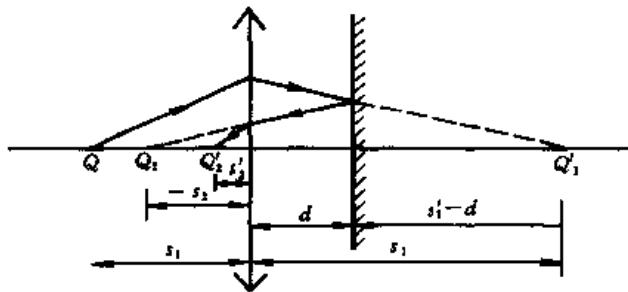
\includegraphics[width=0.3\textwidth]{figures/光图1-19-1.jpg}
\end{center}
\vfill


\textbf{1-20} 如光图1-20-1所示， $L_{1}$ 和 $L_{2}$ 分别为薄凸透镜和薄凹透镜，前面放一小物，移动屏幕到 $L_{2}$ 后  20 cm处, 即 $M_{1}$ 处接收到像. 现将薄凹透镜 $L_{2}$ 撤去,将屏幕移前 5 cm 至 $M_{2}$ 处，重新接收到像。试求薄凹透镜 $L_{2}$ 的焦距 $f_{2}$ .

\begin{center}
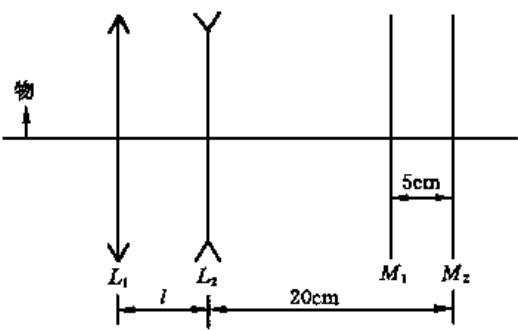
\includegraphics[width=0.3\textwidth]{figures/光图1-20-1.jpg}
\end{center}
\vfill
\newpage

\textbf{1-21} 如光图1-21-1所示是由一个棱镜和两个薄透镜组成的光学系统。棱镜是等腰直角棱镜，腰长 $d = 6\mathrm{cm}$ ，折射率 $n = 1.5$ 。物高 $y = 1\mathrm{cm}$ ，先经棱镜斜面反射，再入射到由 $\mathbf{L}_1$ 和 $\mathbf{L}_2$ 组成的薄透镜系统，两薄透镜的焦距分别为 $f_1 = 20\mathrm{cm}$ 和 $f_2 = -10\mathrm{cm}$ ，它们的间距为 $5\mathrm{cm}, L_1$ 与直角棱镜的距离为 $10\mathrm{cm}$ 。       试求最后像的位置,虚实和正倒.

\begin{center}
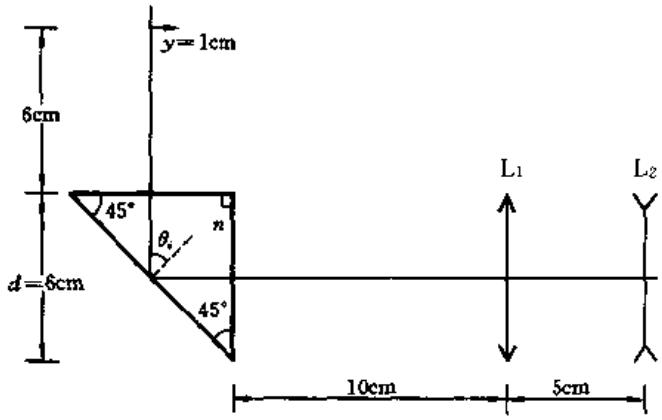
\includegraphics[width=0.3\textwidth]{figures/光图1-21-1.jpg}
\end{center}
\vfill


\textbf{1-22} 如光图1-22-1所示，双凸薄透镜两个球面的曲率半径相同，平放在平面反射镜上，其间充满了水，水的折射率为 $n_{W}$ ，试导出测定透镜折射率的公式，并简述测量方法。

\begin{center}
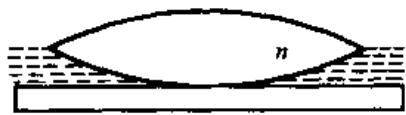
\includegraphics[width=0.3\textwidth]{figures/光图1-22-1.jpg}
\end{center}
\vfill\newpage


\textbf{1-23} 如光图1-23-1所示，两个完全相同的球面薄表壳玻璃合在一起，中空，其中一块涂银成为球面反射镜。屏上小孔 $Q$ 为点光源，它发出的光经反射后成像于 $Q'$ 点。调整屏与表壳玻璃之间的距离 $L$ ，当 $L = 20 \mathrm{~cm}$ 时，像点 $Q'$ 正好落在屏上。然后在表壳玻璃间注满折射率 $n = \frac{4}{3}$ 的水。试问，当 $L$ 为何值时，像点 $Q'$ 仍落在屏上？

\begin{center}
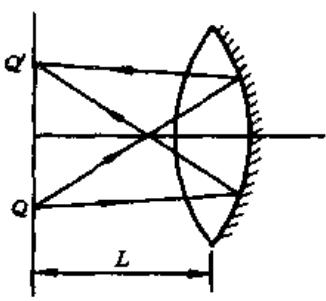
\includegraphics[width=0.3\textwidth]{figures/光图1-23-1.jpg}
\end{center}
\vfill


\textbf{1-24} 如光图1-24-1所示，一个双凸薄透镜的两个球面的曲率半径均为 $r$ ，透镜的折射率为 $n$ ，考察由透镜后表面反射所形成的实像．试问物放于何处，可使反射像与物位于同一平面内（不考虑多重反射）.

\begin{center}
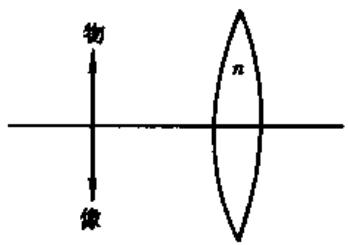
\includegraphics[width=0.3\textwidth]{figures/光图1-24-1.jpg}
\end{center}
\vfill\newpage


\textbf{1-25} 如光图1-25-1所示，在薄壁玻璃水槽的外壁贴着由同种玻璃制成的平凸薄透镜，透镜在空气中的焦距为 $f_{0}$ 。已知水，玻璃，空气的折射率分别为 $n_{1} = \frac{4}{3}, n = \frac{3}{2}, n_{2} = 1$ 。在透镜光轴上距内壁 $s = f_{0}$ 处有一物点 $Q$ 。试求：1. 像的位置和横向放大率。2. 若将透镜贴在水槽内壁，结果如何？

\begin{center}
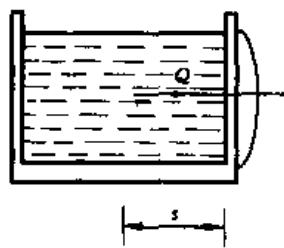
\includegraphics[width=0.3\textwidth]{figures/光图1-25-1.jpg}
\end{center}
\vfill


\textbf{1-26} 已知一薄凸透镜的焦距为 $f$ 。设物是一个半径为 $R$ 的球面，球心在光轴上，试分析像  物理学难题集萃（增订本）  仍为一球面的可能性及条件。

\vfill\newpage


\textbf{1-27} 厚度为 $d$ 的厚透镜放置在空气中，对于波长为 $\lambda_{a}$ 和 $\lambda_{b}$ 的光，该透镜的折射率分别为 $n_{a}$ 和 $n_{b}$ . 试求：1. 该厚透镜主面的位置及有效焦距。2. 为使波长为 $\lambda_{a}$ 和 $\lambda_{b}$ 的两种光有相同的有效焦距，厚透镜两个球面的曲率半径 $r_{1}$ 和 $r_{2}$ 应满足什么关系？

\vfill


\textbf{1-28} 玻璃球的半径为 $r = 2.00\mathrm{cm}$ ，折射率为 $n = 1.50$ ，放置在空气中。1. 试求焦距以及主点和焦点的位置。2. 在球面上有一小物，从另一侧观察，试求像的位置和横向放大率，并作图验证之。

\vfill\newpage


\textbf{1-29} 如光图1-29-1所示，两薄透镜共轴，一为会聚透镜，其焦距为 $f_{1} = 10\mathrm{cm}$ ，另一为发散透镜，其焦距为 $f_{2} = -15\mathrm{cm}$ ，发散透镜位于会聚透镜后 $5\mathrm{cm}$ 处。一物放置在会聚透镜前方 $10\mathrm{cm}$ 处。       试求:透镜组的焦点和主点位置,并求最后像的位置、大小、虚实和正倒.

\begin{center}
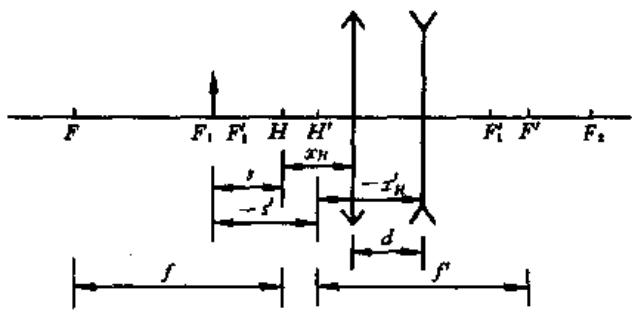
\includegraphics[width=0.3\textwidth]{figures/光图1-29-1.jpg}
\end{center}
\vfill


\textbf{1-30} 为了说明照相机远摄镜(长焦距镜头)的工作原理,讨论以下问题.  

1. 在物距比焦距大得多的条件下, 试证明对于一定距离外的物体, 相机镜头的横向放大率与焦距成正比.  

2. 远摄镜由前方的会聚透镜和后方的发散透镜组成, 其主要作用除成像外, 还可在不改变机身大小的情况下增加焦距, 以增加横向放大率. 试用作图法解释增加焦距的原理.  

3. 已知两透镜间距 $d = 60 \mathrm{~mm}, f_{1} = 76 \mathrm{~mm}, f_{2} = -25 \mathrm{~mm}$ . 试求有效焦距.  

\vfill\newpage

\textbf{1-31} 已知照相机镜头的焦距为 $f'$ ，通光孔径为 $D$ ，物离照相机镜头的距离为 $s$ ，物点在感光片上形成的弥散圆直径不得大于 $l$ ，试导出“景深” $\Delta s$ 的公式，并分析“景深”与各量的关系。

\vfill


\textbf{1-32} 如光图1-32-1所示为一简单望远镜。物镜 $L_{1}$ 的焦距 $f_{1} = 10\mathrm{cm}$ ，孔径 $D_{1} = 4\mathrm{cm}$ ；在物镜 $L_{1}$ 的像方焦点处放置凸透镜 $L_{2}$ ，其焦距 $f_{2} = 2\mathrm{cm}$ ，孔径 $D_{2} = 1.2\mathrm{cm}$ ；目镜 $L_{3}$ 放置在 $L_{2}$ 后 $2\mathrm{cm}$ 处，其焦距 $f_{3} = 2\mathrm{cm}$ ，孔径 $D_{3} = 1.2\mathrm{cm}$ 。       

1. 试求该望远镜出射光瞳的位置和大小.

2. 试简述透镜 $L_{2}$ 的作用.

3. 试讨论该望远镜是否与眼睛相匹配.
\begin{center}
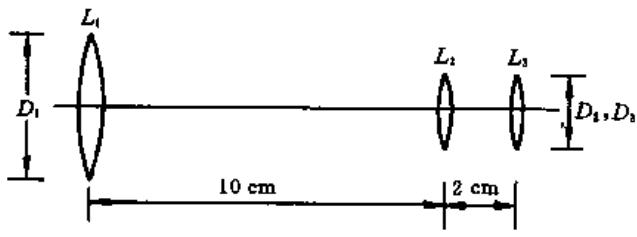
\includegraphics[width=0.3\textwidth]{figures/光图1-32-1.jpg}
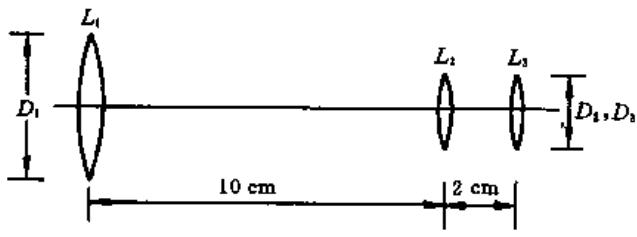
\includegraphics[width=0.3\textwidth]{figures/光图1-32-1.jpg}
\end{center}
\vfill\newpage


\textbf{1-33} 已知显微镜物镜的焦距为 $f_{1} = 2\mathrm{mm}$ ，目镜的焦距为 $f_{2} = 20\mathrm{mm}$ ，光学筒长 $\Delta = 153\mathrm{mm}$ ，最后像离目镜的距离为明视距离 $s_0 = 250\mathrm{mm}$ 。试求：

1.物离物镜的距离。

2.显微镜的视角放大率。

3.显微镜的焦深。

\vfill


\textbf{1-34} 惠更斯目镜由向场镜 $L_{1}$ 和接目镜 $L_{2}$ 组合而成， $L_{1}$ 和 $L_{2}$ 的焦距 $f_{1}$ 和 $f_{2}$ 以及两透镜的间隔 $d$ 满足 $f_{1}: f_{2}: d = 3:1:2$ 。光阑 AA 位于两透镜之间的正中央处， $L_{1}$ 和 $L_{2}$ 以及光阑的孔径直径依次为 $D_{1}$ 和 $D_{2}$ 以及 $D$ 。  试问:

1. 为使 $L_{1}$ 成为孔径光阑, AA 成为视场光阑, 有关孔径的大小应满足什么条件? 

2. 在上述条件下, 计算出射光瞳的位置和大小.

\vfill\newpage


\textbf{1-35} 试证明，在傍轴条件下，显微镜数值孔径一定时，其出射光瞳的直径与显微镜的视角放大率成反比。

\vfill

\textbf{1-36} 已知冕牌玻璃对可见光波段的平均折射率为 $n_0 = 1.499$ ，在 $\Delta \lambda = 170.0 \mathrm{~nm}$ 范围内的平均色散率为 $\frac{\mathrm{d}n_0}{\mathrm{d}\lambda} = -4.74\times 10^{-5}\mathrm{nm}^{-1}$ .火石玻璃的相应数据为 $n_f = 1.610,\frac{\mathrm{d}n_f}{\mathrm{d}\lambda} = -9.76\times$ $10^{-5}\mathrm{nm}^{-1}$ .今用这两种玻璃制成透镜，胶合起来做成消色差透镜．试证明：

1. 两种透镜的焦距必须满足
$$
\frac {\Delta_ {c}}{f _ {c}} + \frac {\Delta_ {f}}{f _ {f}} = 0
$$
式中 $f_{c}$ 为冕牌玻璃透镜的焦距， $f_{f}$ 为火石玻璃透镜的焦距， $\Delta$ 为
$$
\Delta = \frac {1}{n - 1} \frac {\mathrm{d} n}{\mathrm{d} \lambda} \Delta \lambda
$$
即
$$
\Delta_ {c} = \frac {1}{n _ {c} - 1} \frac {\mathrm{d} n _ {c}}{\mathrm{d} \lambda} \Delta \lambda , \quad \Delta_ {f} = \frac {1}{n _ {f} - 1} \frac {\mathrm{d} n _ {f}}{\mathrm{d} \lambda} \Delta \lambda
$$

2. 只有用冕牌玻璃做成会聚透镜, 用火石玻璃做成发散透镜, 才有可能得到会聚的消色差镜头.

\vfill
\newpage

\textbf{1-37} 两个分离的薄透镜组合成透镜组，它们的焦距分别为 $f_{1}$ 和 $f_{2}$ ，在所使用的光波波段内的平均折射率分别为 $n_{1}$ 和 $n_{2}$ ，平均色散率分别为 $D_{1}$ 和 $D_{2}$ . 试问：为使透镜组具有最小的色差，两透镜的间隔应为多大？

\vfill


\textbf{1-38} 用两个薄会聚透镜组装成一架简易开普勒望远镜，要求该望远镜能分辨 $100\mathrm{m}$ 远物面上 $1\mathrm{mm}$ 间隔的两条刻线。已知镜筒长度（两薄透镜之间的距离）为 $62~\mathrm{cm}$ ，已知人眼的最小分辨角为 $3\times 10^{-4}\mathrm{rad}$ 。  试问:1. 物镜直径应选多大? 2. 物镜和目镜的焦距各为多少? 3. 当目镜直径选用 2 cm 时,望远镜的视场角是多少?

\vfill\newpage


\textbf{1-39} 均匀发光圆盘的半径为 $R$ ，亮度为 $B$ .试计算其中垂轴上与盘心相距为 $z$ ，与轴垂直的面上的照度．设圆盘为朗伯体.

\vfill


\textbf{1-40} 透镜主光轴上一发光小物的亮度为 $B$ ，透镜物方折射率为 $n$ ，像方折射率为 $n'$ ，透镜的透光系数（出射光通量与入射光通量之比）为 $k$ 。试求像的亮度。设发光小物为朗伯体。

\vfill\newpage


\textbf{1-41} 试证明,用照相机拍摄远物时,感光片上像的照度与物的远近基本无关,而与镜头的相对孔径的平方成正比.

\vfill


\textbf{1-42} 正入射的太阳光照射到一屏幕上，另用一半径为 $r$ 、焦距为 $f$ 的透镜将太阳光聚焦在屏幕上。试求上述两种情形下的照度之比。又，对于一定的 $r$ ，试问 $f$ 为何值时，两种情形的照度相等。设太阳为朗伯体，观察太阳的视角为0.01 rad。设透镜的透光系数为1。

\vfill
